%============================== Setting teh Document=============================================

\documentclass{beamer}
\usepackage[italian]{babel} 
\usepackage[latin1]{inputenc} 
\usepackage[T1]{fontenc}
\usepackage{graphicx} 
\usetheme{Madrid} 


%==========================Set the foot line========================================================
\makeatletter
\setbeamertemplate{footline}
{
  \leavevmode%
\hbox{%
	\begin{beamercolorbox}[wd=.333333\paperwidth,ht=2.25ex,dp=1ex,center]{author in head/foot}%
	\usebeamerfont{author in head/foot}\insertsection
\end{beamercolorbox}%
\begin{beamercolorbox}[wd=.333333\paperwidth,ht=2.25ex,dp=1ex,center]{title in head/foot}%
	\usebeamerfont{title in head/foot}\insertsubsection
\end{beamercolorbox}%
\begin{beamercolorbox}[wd=.333333\paperwidth,ht=2.25ex,dp=1ex,right]{date in head/foot}%
	\usebeamerfont{date in head/foot}\insertshortdate{}\hspace*{2em}
	\insertframenumber{} / \inserttotalframenumber\hspace*{2ex} 
\end{beamercolorbox}}%
}%
\vskip0pt%

\makeatother



\title{Analisi della struttura sanitaria della provincia di Ascoli Piceno} 
\author{Enrico Ferretti \\ 
		Tommaso Cicco\\
		Francesco Rombaldoni\\
		} 
\institute{Universit� degli Studi di Urbino "Carlo Bo"} 
\logo{\includegraphics[width=15mm]{Uni}}

%\useoutertheme[right]{sidebar} 
\setbeamercovered{dynamic}

%=========================================== Starting Document=====================================
\begin{document}

	\begin{frame} 
		\maketitle 		
	\end{frame}

	\begin{frame} 
		\frametitle{Indice} 
		\tableofcontents 
	\end{frame}

	\section{Presentazione}
	\begin{frame} 
		\frametitle{Obbiettivo:} 
	%	\framesubtitle{Sottotitolo} 
	L'obbiettivo dell'analisi � di determinare se la rete delle strutture della provincia di Ascoli Piceno che erogano servizi d'assistenza psichiatrica corrisponde a una delle seguenti strutture ed il cambiamento negli anni 2015, 2017, 2019:  
	
	\bigskip
	
	\begin{enumerate}
		\item Organizzazione diffusa.
		\item Organizzazione centralizzata.
		\item Organizzazione Integrata
	\end{enumerate}

\end{frame}

%----------------------Staring report part-----------------------------

\section{Operazioni Svolte}

\begin{frame}
	\frametitle{Operazioni svolte}
	I grafi, che rappresentano la struttura della rete, sono stati generati tramite il software Gephi; sono state inoltre svolte le seguenti operazioni:
	\bigskip
	\begin{enumerate}
		\item Determinazione della centralit� relativa alla closeness.
		\item Calcolo della centralizzazione dei grafi.
		\item Determinazione del "K-Core".
	\end{enumerate}
\end{frame}
%===========================================2015=====================================
\section{Anno 2015}

\addtocontents{toc}{\protect\setcounter{tocdepth}{1}}
\subsection{Statistiche generali}
\begin{frame}
	\frametitle{Anno 2015}
	\framesubtitle{Statistiche generali}
	\begin{itemize}
		\item Rete formata da 25 nodi e 79 archi.
		\item Il nodo pi� centrale � "CSM Ospedale AP".
		\item Centralizzazione del grafo: 49\%.
		\item Unica componente connessa.
	\end{itemize} 
\end{frame}

\subsection{Grafo generato}
\begin{frame}
	\frametitle{Anno 2015}
	\framesubtitle{Grafo generato}
	\begin{figure}
		\centering
		\caption{Grafo generato applicando gli algoritmi "Force Atlas 2" ed "Expansion".}
		\label{fig:graph2015}
		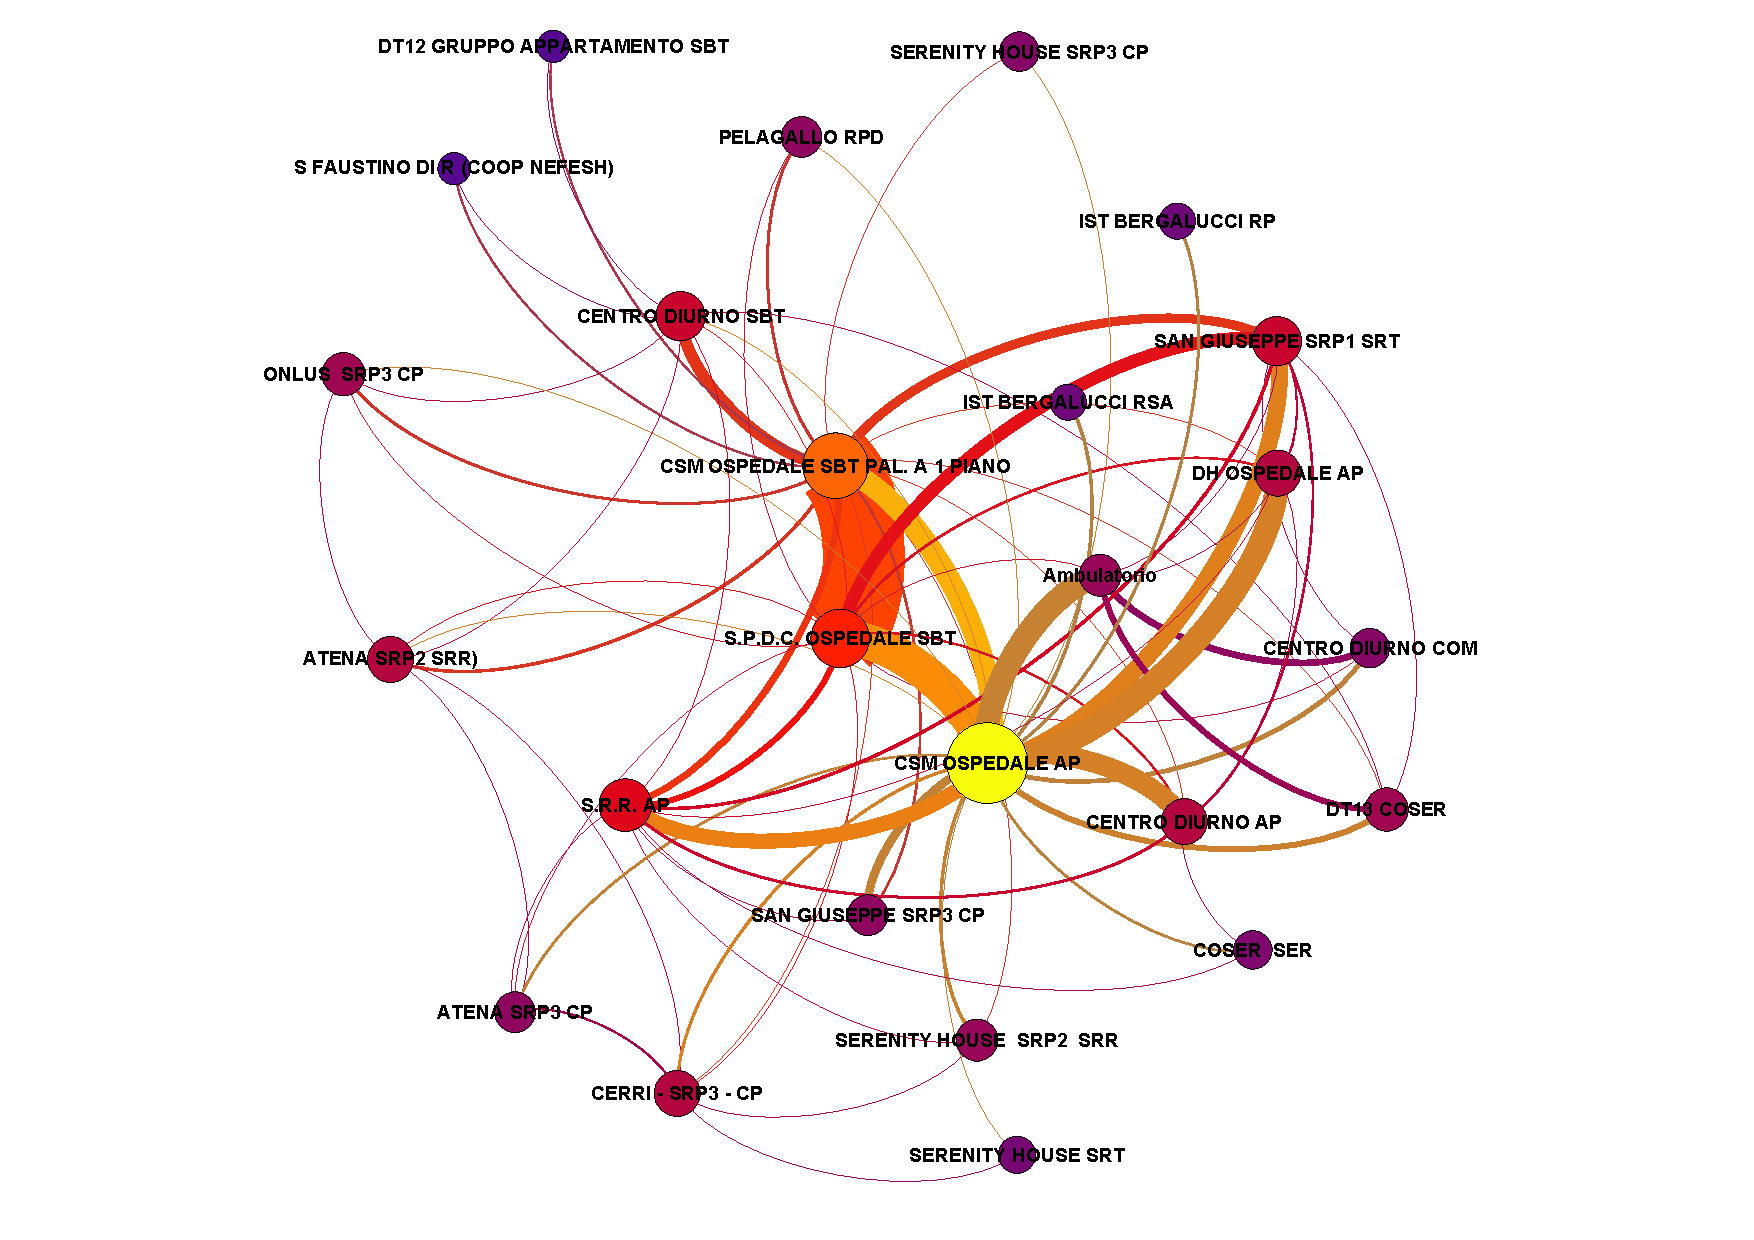
\includegraphics[width=0.7\linewidth]{imgs/Graph_2015}
	\end{figure}
\end{frame}

\subsection{K-Core}
\begin{frame}
	\frametitle{Anno 2015}
	\framesubtitle{K-Core}
	\begin{figure}
		\centering
		\caption{"K-Core" per K = 6 del grafo.}
		\label{fig:kcore2015}
		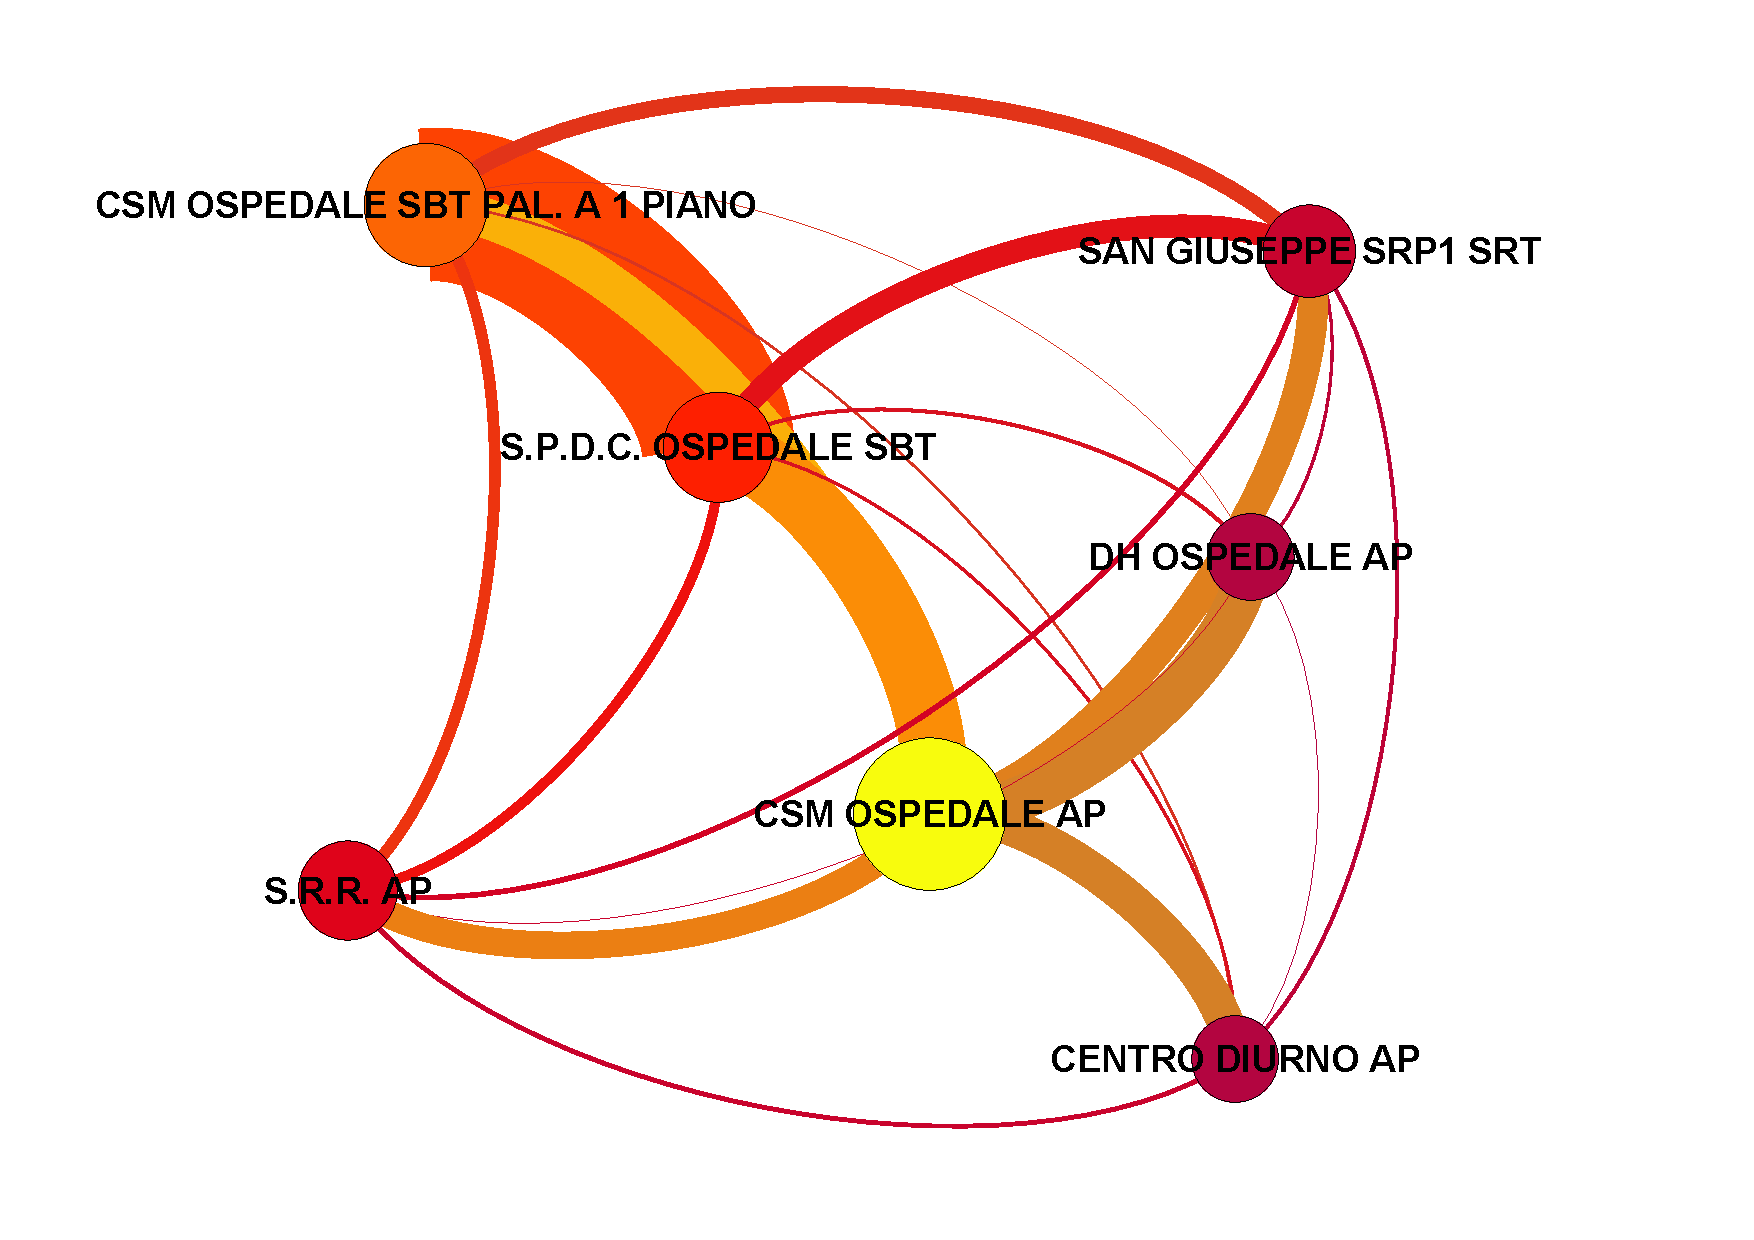
\includegraphics[width=0.7\linewidth]{imgs/K-core_2015}
	\end{figure}
\end{frame}

\subsection{Centralit�}
\begin{frame}
	\frametitle{Anno 2015}
	\framesubtitle{Centralit�}
	\begin{figure}
		\centering
		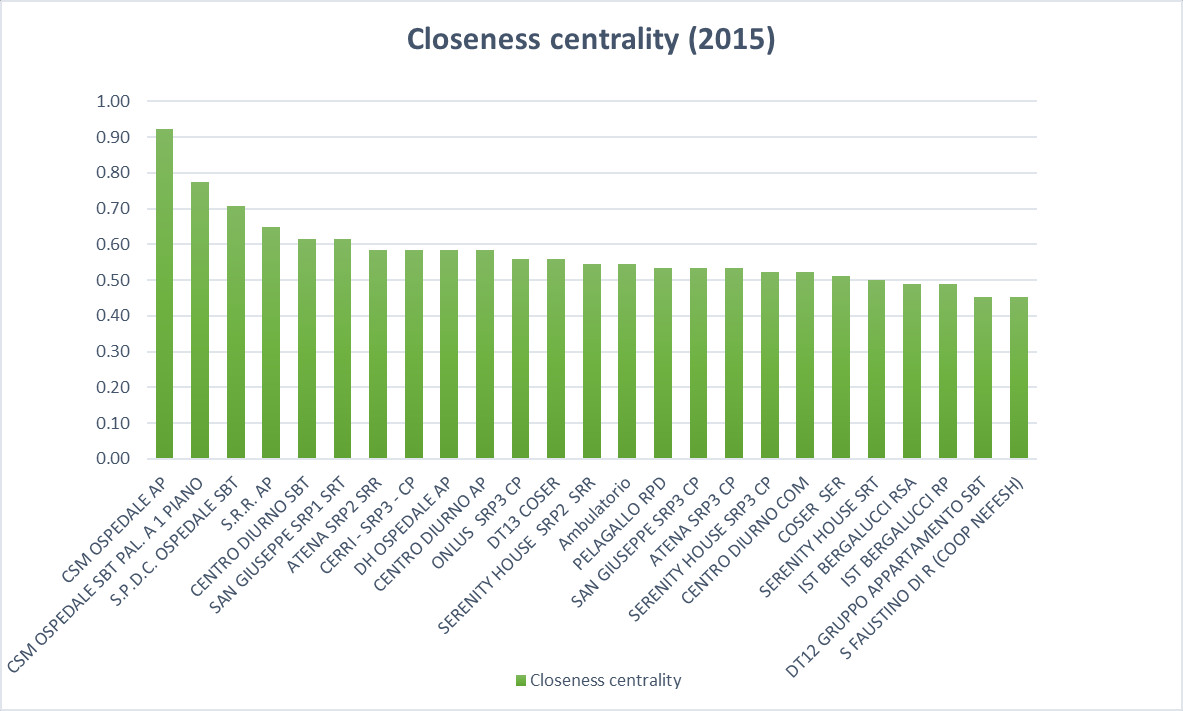
\includegraphics[width=0.8\linewidth]{imgs/2015_diagram}
		\label{fig:2015diagram}
	\end{figure}
\end{frame}

\subsection{Analisi}
\begin{frame}
	\frametitle{Anno 2015}
	In conclusione la rete del 2015 � identificabile come una rete integrata, siccome � organizzata attorno ad un nucleo di strutture, tra le quali spicca l'ospedale "CSM" di Ascoli Piceno.\\
	\bigskip
	Il "K-Core" di grado 6 (grado massimo) mostra un nucleo composto da 7 strutture che sono in stretta collaborazione tra di loro.\\
\end{frame}


%============================================================2017==========================================================
\section{Anno 2017}

\subsection{Statistiche generali}
\begin{frame}
	\frametitle{Anno 2017}
	\framesubtitle{Statistiche generali}
	\begin{itemize}
		\item Rete formata da 31 nodi e 94 archi.
		\item Il nodo pi� centrale � "CSM Ospedale AP".
		\item Centralizzazione del grafo: 38\%.
		\item Nodo isolato: "Atena SRP3 CP". 
	\end{itemize} 
\end{frame}

\subsection{Grafo generato}
\begin{frame}
	\frametitle{Anno 2017}
	\framesubtitle{Grafo generato}
	\begin{figure}
		\centering
		\caption{Grafo generato applicando gli algoritmi "Force Atlas 2" ed "Expansion".}
		\label{fig:graph2017}
		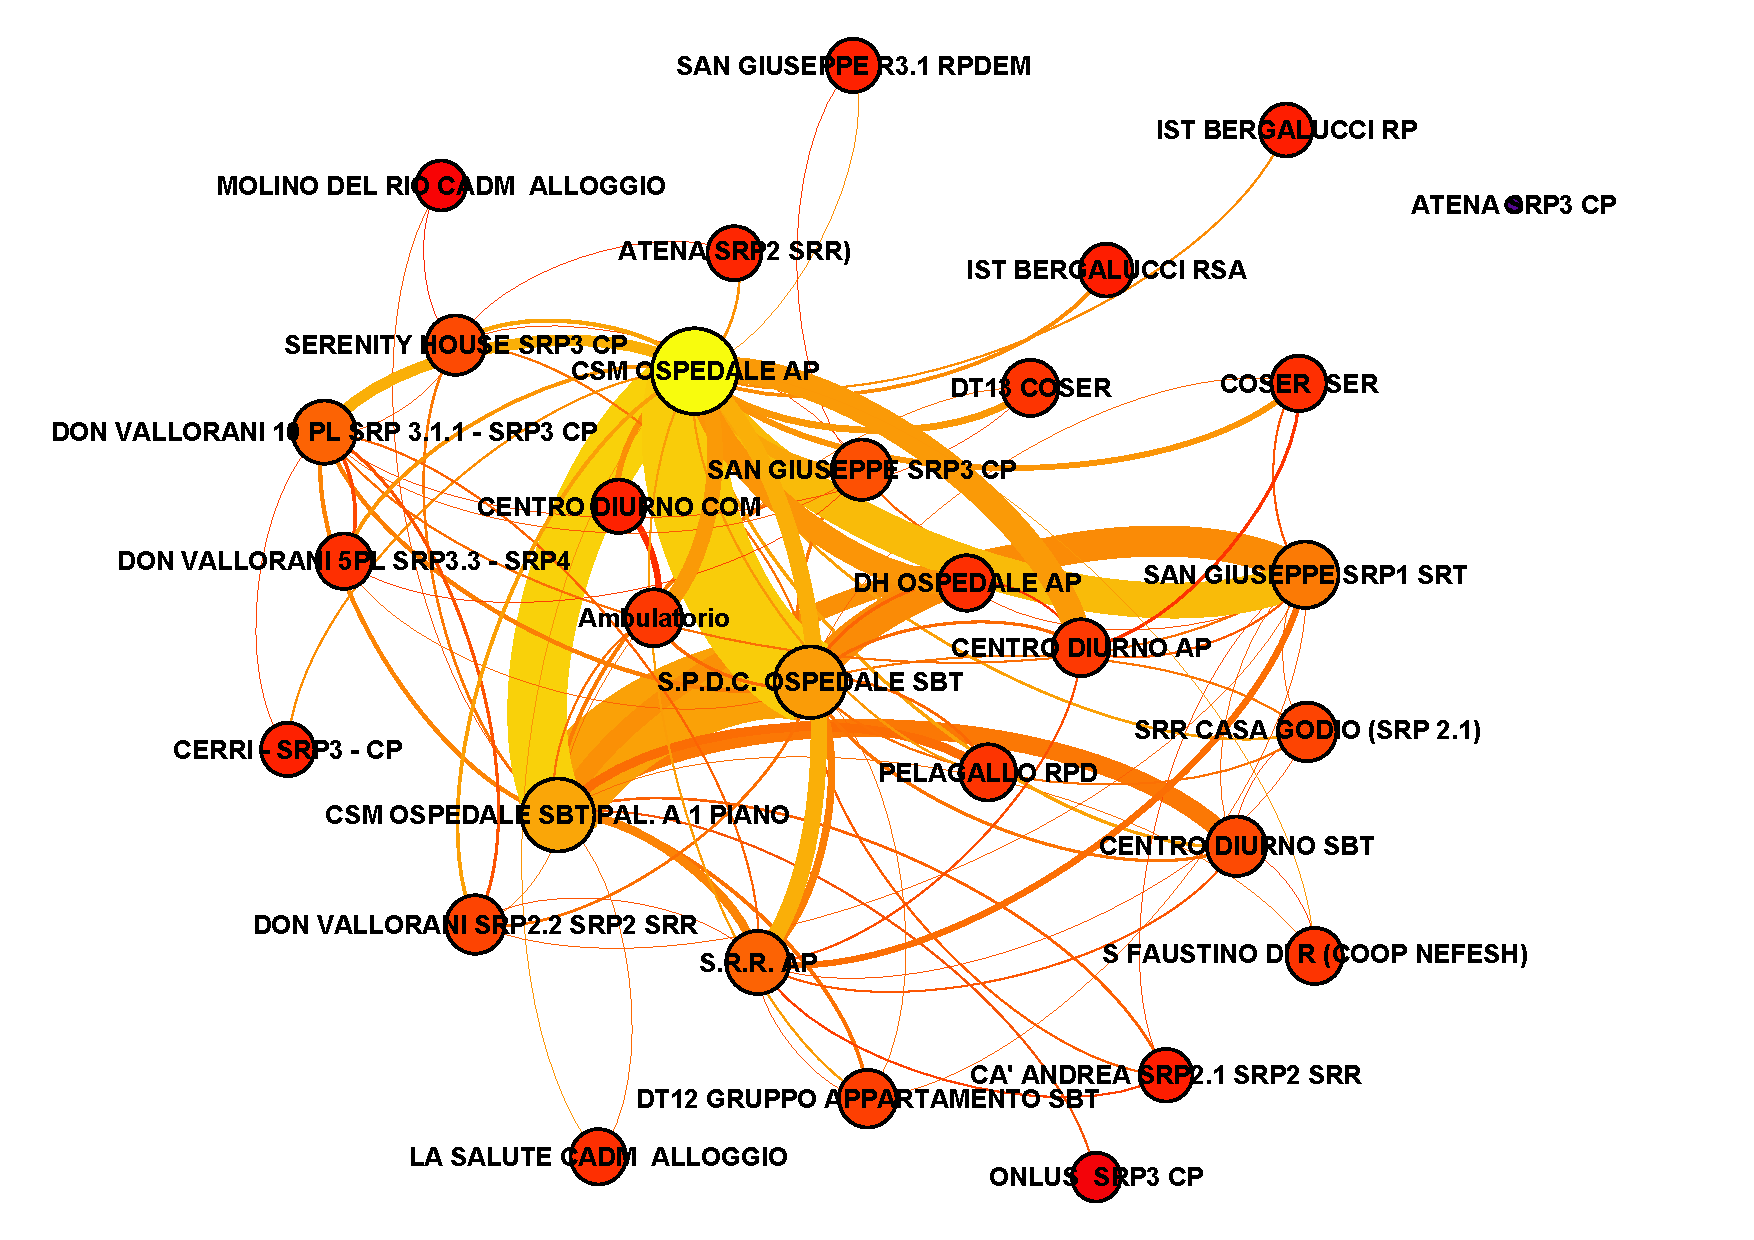
\includegraphics[width=0.7\linewidth]{imgs/Graph_2017}
	\end{figure}
\end{frame}

\subsection{K-Core}
\begin{frame}
	\frametitle{Anno 2017}
	\framesubtitle{K-Core}
	\begin{figure}
		\centering
		\caption{"K-Core" per K = 6 del grafo.}
		\label{fig:kcore2017}
		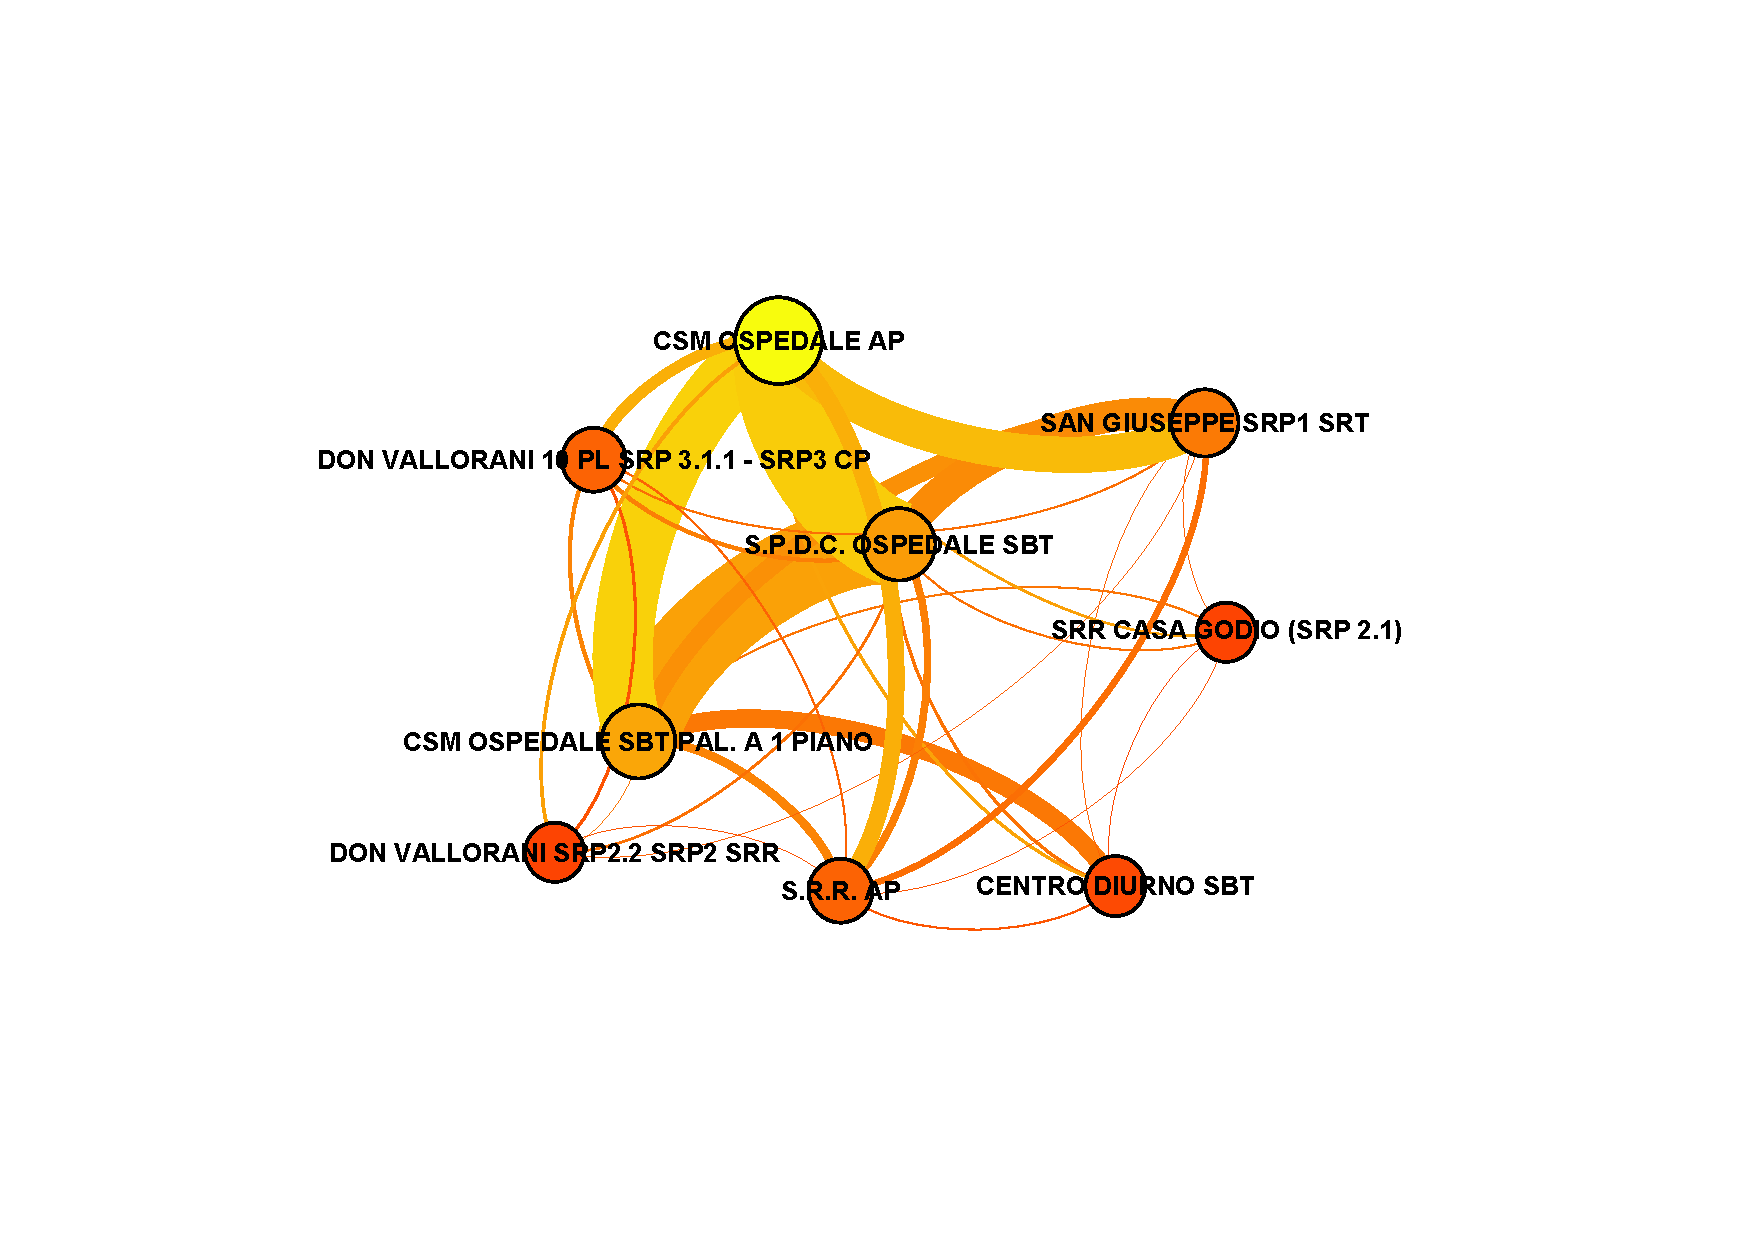
\includegraphics[width=0.7\linewidth]{imgs/K-core_2017}
	\end{figure}
\end{frame}

\subsection{Centralit�}
\begin{frame}
	\frametitle{Anno 2017}
	\framesubtitle{Centralit�}
	\begin{figure}
		\centering
		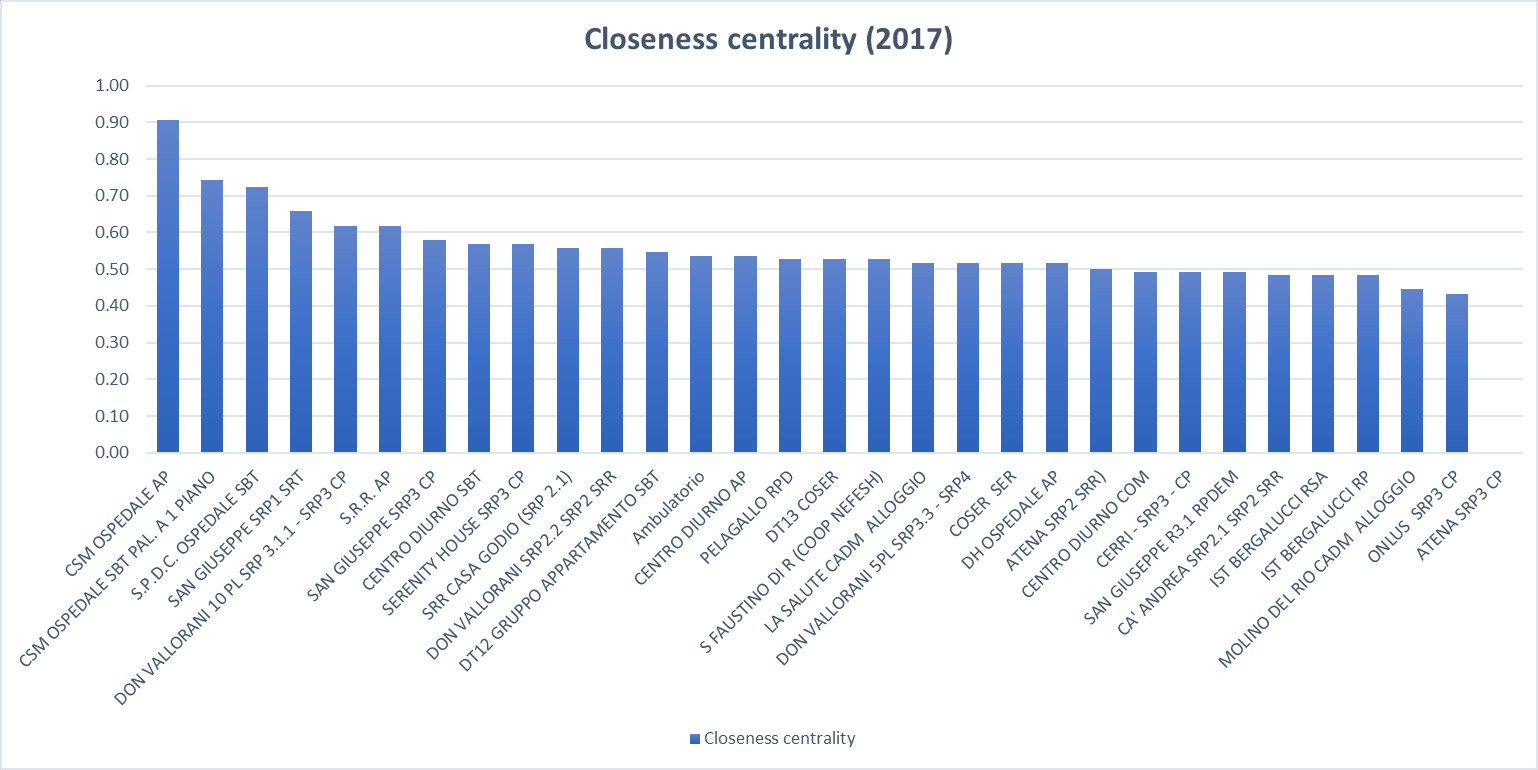
\includegraphics[width=0.8\linewidth]{imgs/2017_diagram}
		\label{fig:2017diagram}
	\end{figure}
\end{frame}


\subsection{Analisi}
\begin{frame}
	\frametitle{Anno 2017}
	La rete del 2017 si avvicina ad una rete diffusa, siccome ci sono meno differenze in termini di centralit� tra i nodi, pur mantenendo un nucleo centrale tipico della rete integrata.\\
	\bigskip
	Il "K-Core" di grado 6 (grado massimo) mostra un nucleo composto da 9 strutture.\\
	Rispetto al 2015 � aumentata la collaborazione.\\
\end{frame}



%==============================================2019==============================
\section{Anno 2019}

\subsection{Statistiche generali}
\begin{frame}
	\frametitle{Anno 2019}
	\framesubtitle{Statistiche generali}
	\begin{itemize}
		\item Rete formata da 31 nodi e 105 archi.
		\item Il nodo pi� centrale � "CSM Ospedale SBT (Pal.A 1� piano)".
		\item Centralizzazione del grafo: 52\%. 
		\item Unica componente connessa.
	\end{itemize} 
\end{frame}

\subsection{Grafo generato}
\begin{frame}
	\frametitle{Anno 2019}
	\framesubtitle{Grafo generato}
	\begin{figure}
		\centering
		\caption{Grafo generato applicando gli algoritmi "Force Atlas 2" ed "Expansion".}
		\label{fig:graph2019}
		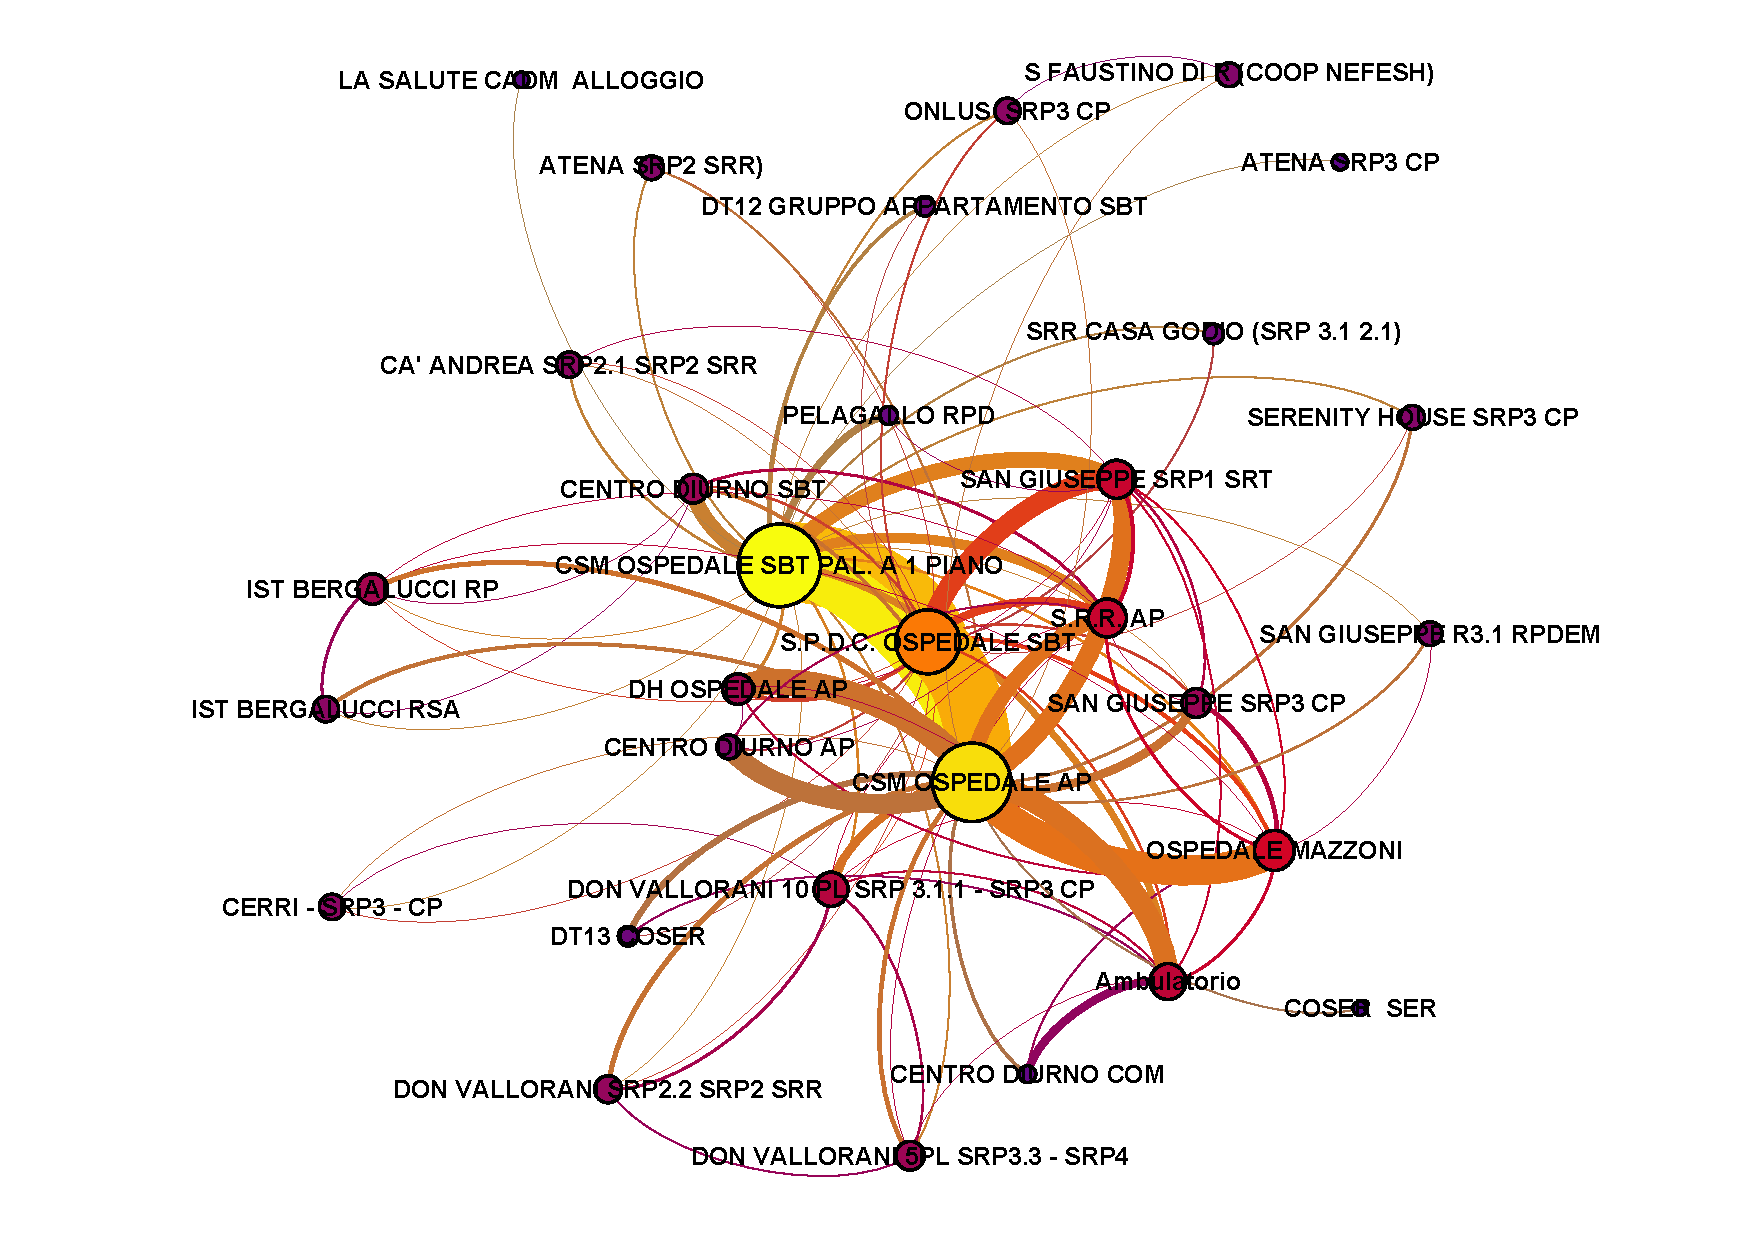
\includegraphics[width=0.7\linewidth]{imgs/Graph_2019}
	\end{figure}
\end{frame}

\subsection{K-Core}
\begin{frame}
	\frametitle{Anno 2019}
	\framesubtitle{K-Core}
	\begin{figure}
		\centering
		\caption{"K-Core" per K = 6 del grafo.}
		\label{fig:kcore2019}
		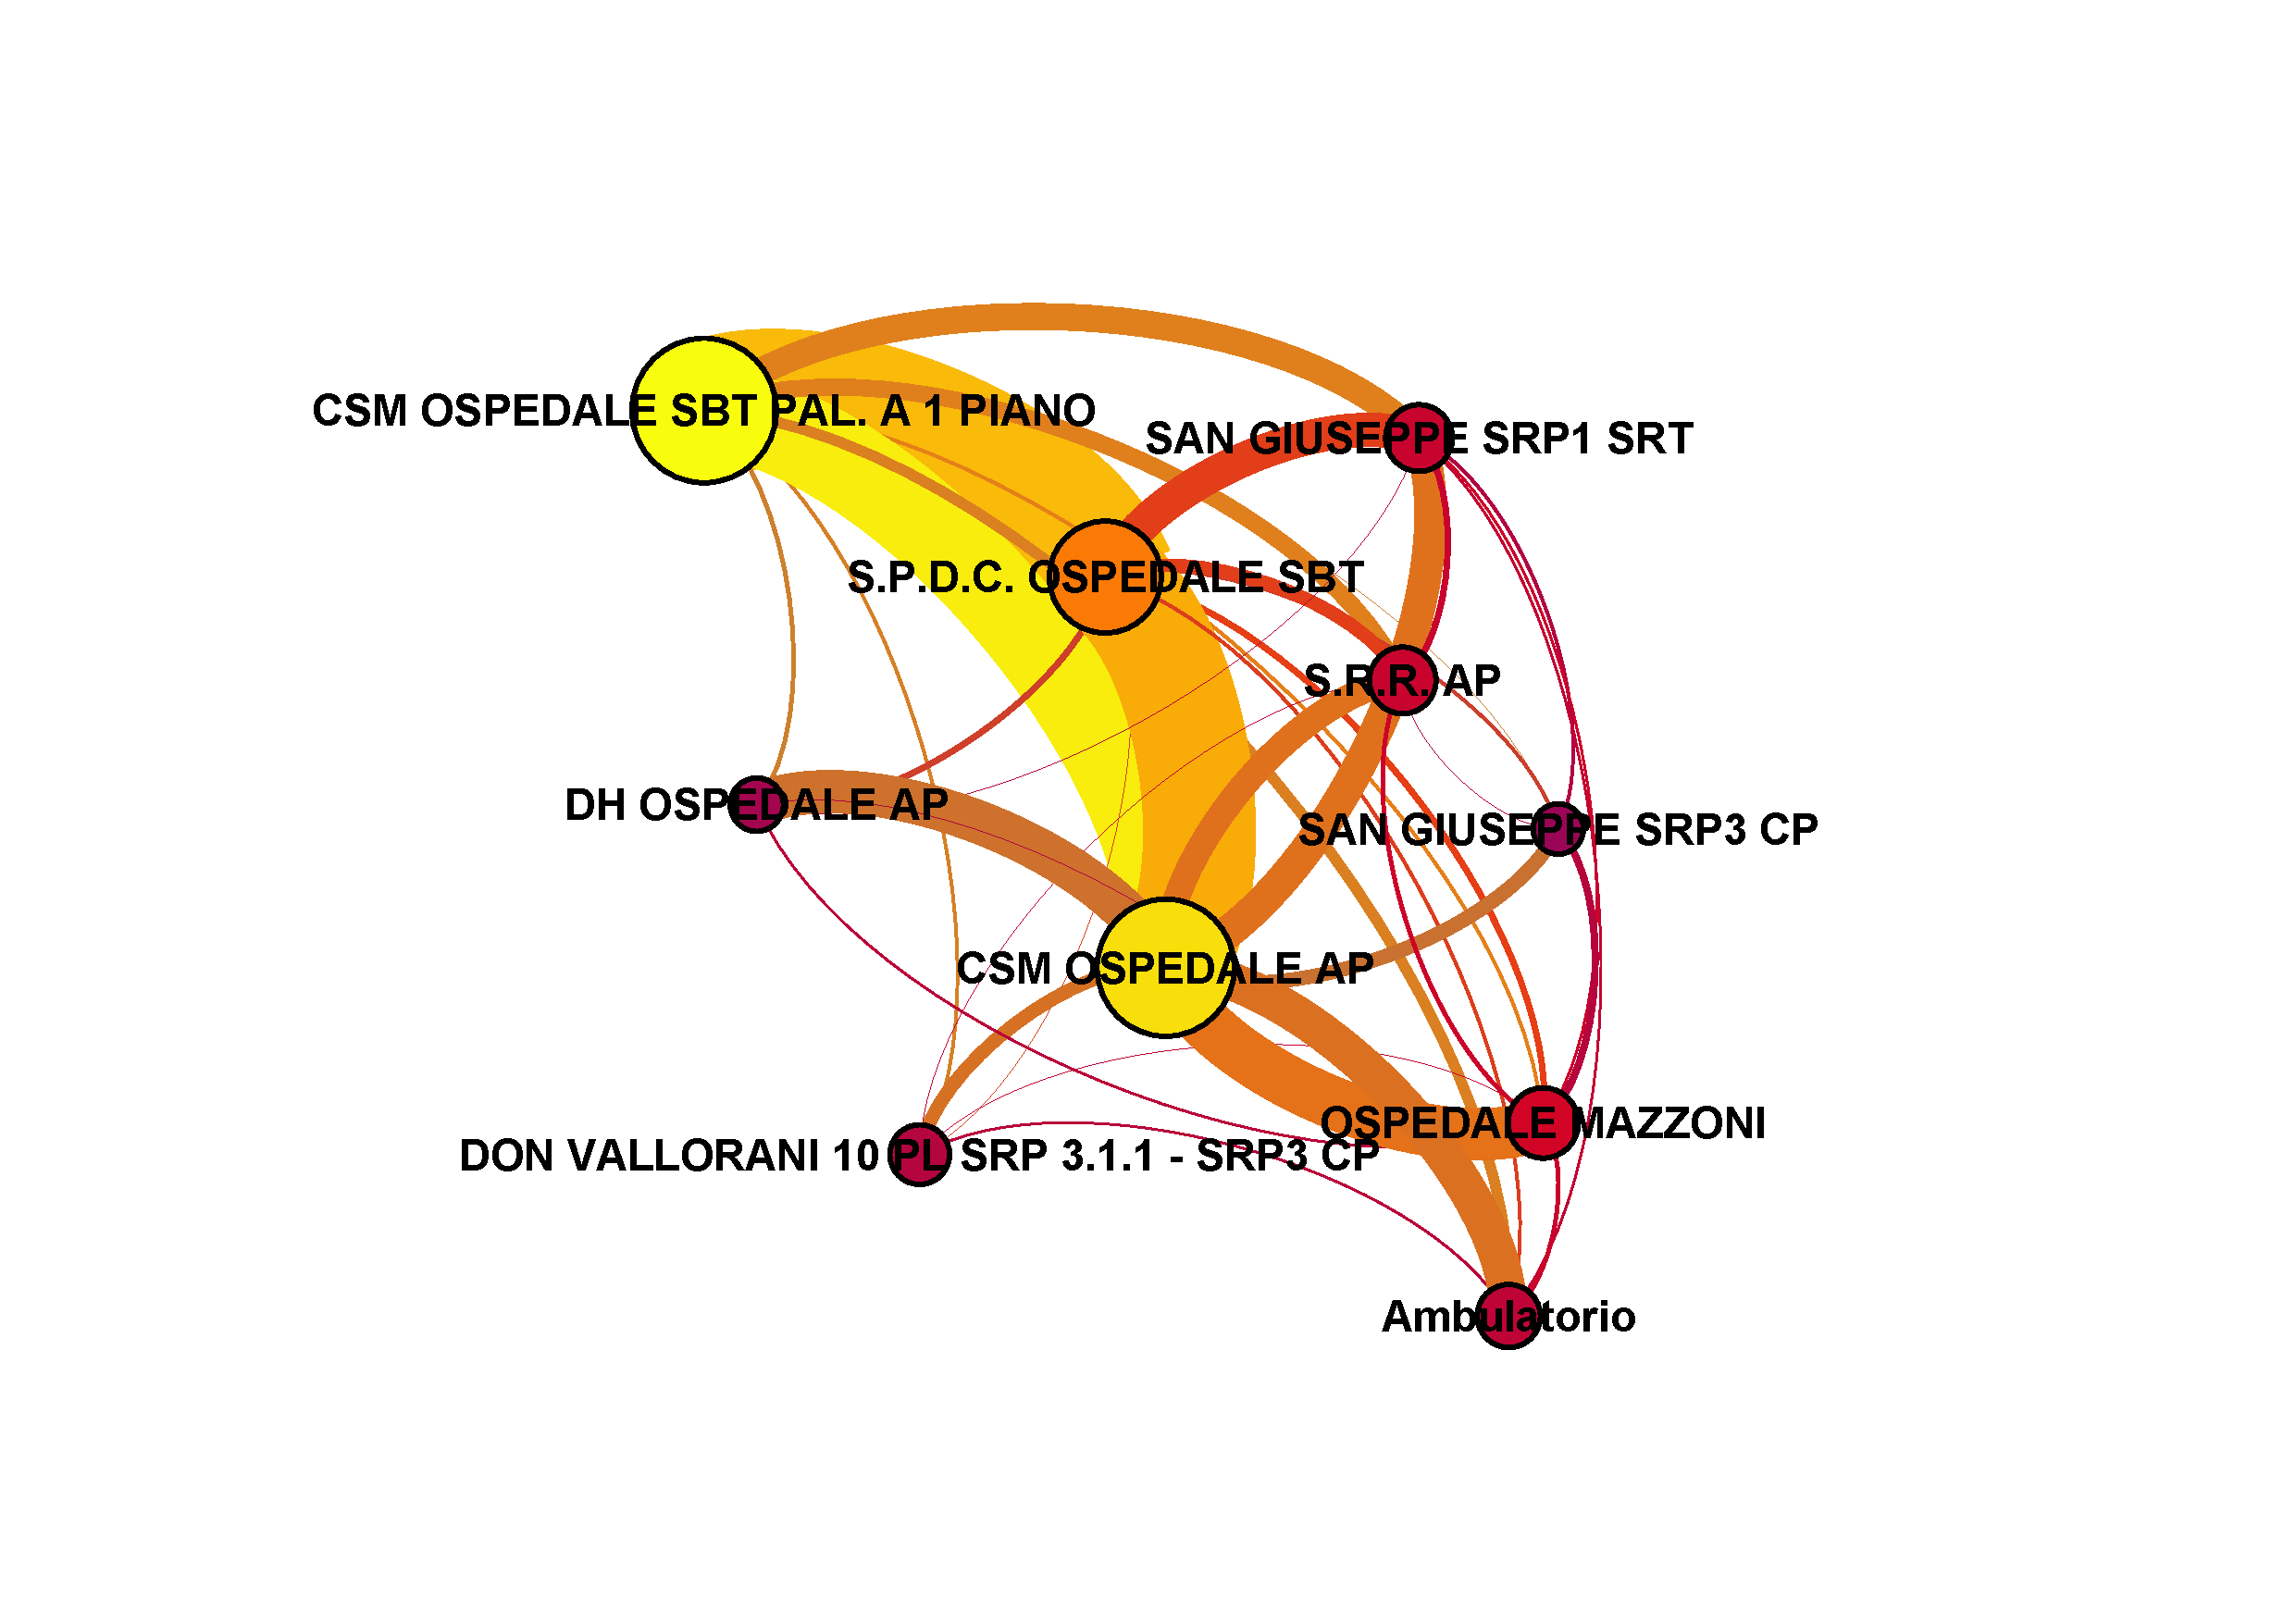
\includegraphics[width=0.7\linewidth]{imgs/K-core_2019}
	\end{figure}
\end{frame}

\subsection{Centralit�}
\begin{frame}
	\frametitle{Anno 2019}
	\framesubtitle{Centralit�}
	\begin{figure}
		\centering
		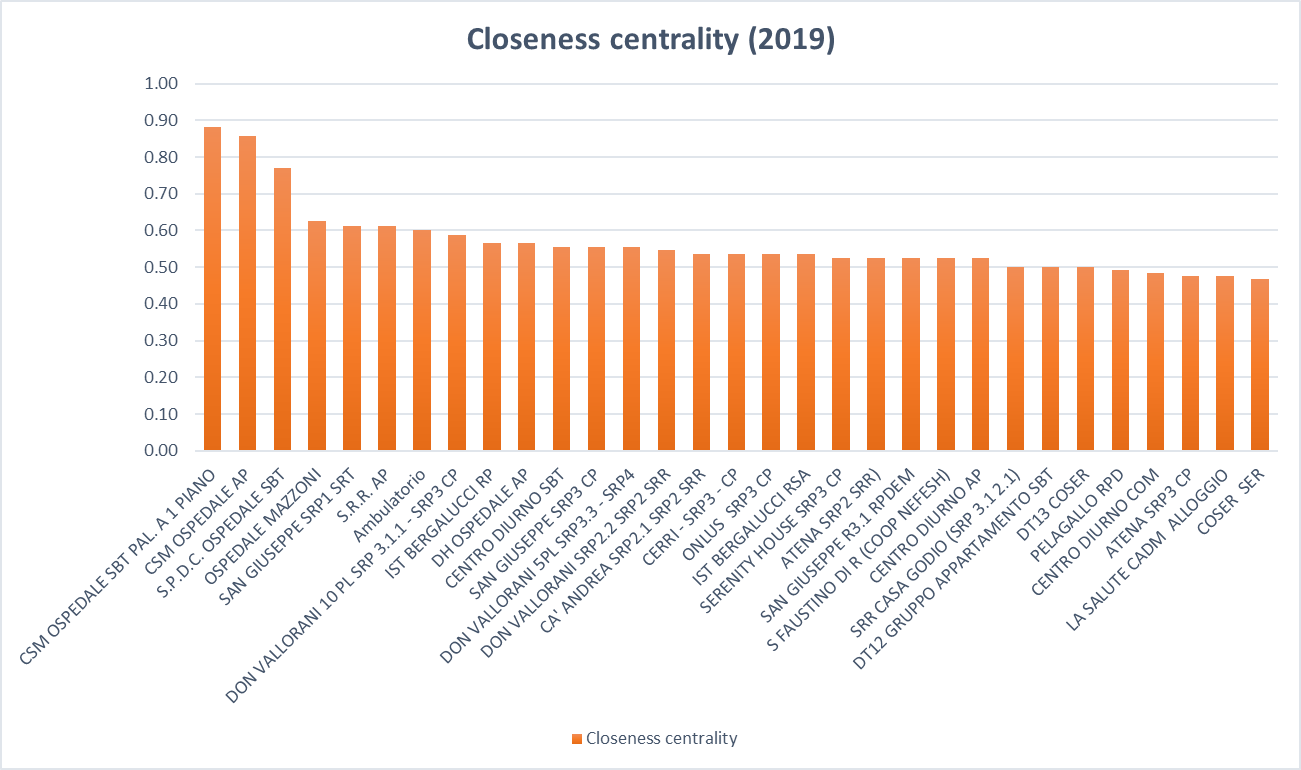
\includegraphics[width=0.8\linewidth]{imgs/2019_diagram}
		\label{fig:2019diagram}
	\end{figure}
\end{frame}


\subsection{Analisi}
\begin{frame}
	\frametitle{Anno 2019}
	Nel 2019 la rete ospedaliera ritorna ad essere una rete integrata, simile a quella del 2015. In particolare rispetto alle precedenti reti � la pi� centralizzata, siccome � presente una maggiore disparit� tra le strutture principali del nucleo e quelle secondarie.\\ 
	\bigskip
	Il "K-Core" di grado 6 (grado massimo) mostra un nucleo composto da 11 strutture.\\
	Rispetto al 2017 � aumentata la collaborazione.\\
\end{frame}

\section{Conclusioni}
%\subsection{Conclusioni}
	\begin{frame}
	\frametitle{Conclusioni}
	In conclusione si evince che nei tre periodi analizzati il nucleo individuato dal "K-Core" di grado 6 � aumentato nel numero delle strutture e dei collegamenti, per cui la collaborazione � aumentata.\\
	Inoltre si pu� notare come l'ospedale di Ascoli Piceno � rimasto tra i nodi coordinatori in tutti gli anni analizzati.\\
	\bigskip
	Nel 2017 l'ospedale "Atena-SRP", non presente nel 2015, � un nodo isolato in quanto � una nuova struttura, che nel 2019 entra in relazione con "CSM-Ospedale-SBT".\\ 
	
	\end{frame}

\begin{frame}
	\frametitle{Conclusioni}
	La gestione della rete ospedaliera � dipendente da due fattori: la necessit� di cure per la salute mentale e l'ammontare dei  fondi stanziati dalla regione Marche.\\
	In particolare maggiori sono i fondi maggiore � la diffusione della rete poich� le strutture riescono a distribuirsi meglio i pazienti.\\
\end{frame}

%============================== Eding document=====================================================
\end{document}




